\section{Detailed design} \label{s:general-approach:detailed-design}
	\gls{gitlab} application deployed on \gls{AWS} can be used in various ways. The very easy and the less optimal/safety way is to deploy every components from Figure \ref{fig:multiple-application-servers} on the same machine. Such approach reduces the latency of retrieving data from but increases the uptime and overall response time.
	
	Approach presented in this section ensure redundancy and minimize inbound connectivity of components to specific ports. As described in Figure \ref{fig:detailed-design} it is possible to distinguish two subnets inside \gls{VPC}:
	\begin{itemize}
		\item public -- \gls{gitlab} web servers;
		\item private -- components required for application (\gls{redis}, \gls{SQLDBMS} and file system for \gls{git})
	\end{itemize}	
	\begin{figure}[!htbp]
		\centering
		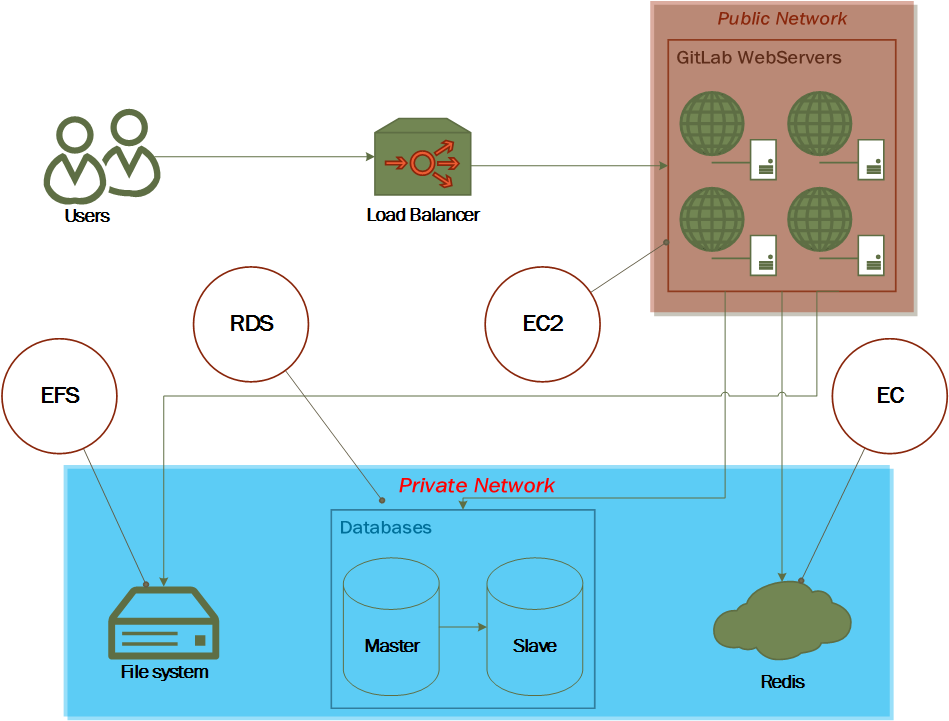
\includegraphics[width=1\textwidth]{img/detailed-model2}
		\caption{Detailed design of \gls{gitlab} deployment on \gls{AWS}.}
		\label{fig:detailed-design}
	\end{figure}
	Application makes use of four \gls{AWS}es, such as:
	\begin{itemize}
		\item
		{
			\gls{RDS} -- for PostgreSQL Databases;
		}
		\item
		{
			\gls{EFS} -- for \gls{git} file system;
		}
		\item
		{
			\gls{EC} -- elastic cache using \gls{redis};
		}
		\item
		{
			\gls{EC2} -- for web servers.
		}
	\end{itemize}

	Public subnet contains up to four (provided by \gls{EC2}) instances of the same \gls{gitlab} servers depending of the CPU utilization. If usage of CPU reach $60\%$ for at least 5 minutes there will be added one new instance. If usage of CPU will be at the level of $40\%$ or less for more than 5 minutes the instance will be terminated. The same approach is used in case if any of running instances will crash.
	
	In private subnet accessing the components is allowed only for others within the same \gls{VPC} subnet. File system running on \gls{EFS} is separated in two different regions similarly to databases and web--servers. PostgreSQL are regularly backed up and additionally there is created redundant read-only slave database, which is a secondary database in case of crash the master one. All mentioned featured are available by \gls{RDS}. \gls{redis} is third and the last component in private subnet it is a caching system for the data structures used by \gls{gitlab} provided by \gls{EC} features from the \gls{AWS}. In case of emergency web-servers can be run using build-in \gls{redis} solution.
	
	Table \ref{tab:security-groups} presents set of inbound rules used in components of the \gls{gitlab} application. According to this table and Figure \ref{fig:detailed-design} it is clear that source of the private subnet components requests are only \gls{EC2} instances situated in public part of \gls{VPC}.
	\begin{table}[!htbp]
		\centering
		\caption{Security groups inbound rules.}
		\label{tab:security-groups}
		\begin{tabular}{|l|l|l|}
			\hline
			\multicolumn{1}{|c|}{\textbf{Security Group}} & \multicolumn{1}{c|}{\textbf{Inbound Rules}} & \multicolumn{1}{c|}{\textbf{Source}} \\ \hline
			EC - Redis & Custom TCP 6379 & EC2 - GitLab \\ \hline
			EC2 - GitLab & HTTP TCP 80 & 0.0.0.0/0 \\ \hline
			EFS - GitLab & NFS TCP 2049 & EC2 - GitLab \\ \hline
			LB - GitLab & HTTP TCP 80 & 0.0.0.0/0 \\ \hline
			RDS - GitLab & PostgreSQL TCP 5432 & EC2 - GitLab \\ \hline
		\end{tabular}
	\end{table}
	
	Load balancer checks ping time every $30$ seconds. If in two consecutive pings time is above 5 sec the instance will be considered as unhealthy and in the end as out of service.
	
	All the necessary configuration changes were extracted and are presented in Listening \ref{lst:rb}. There is an information about application url address, configuration of the connection to database, \gls{redis} host name, and mount points to \gls{EFS}. Configuration also disables local PostgreSQL database and \gls{redis}. Mount points are also stored in \emph{fstab} and is presented in Listening \ref{lst:fstab} and are connected to the \gls{gitlab} configuration itself.